\section{Implementation}
\label{sec:sidekick:implementation}

\begin{table}[ht]
  \centering
  \begin{tabular}{l r r}
    \hline
    \textbf{Module} & \textbf{Language} & \textbf{LOC} \\
    \hline
    QuACK library (\Cref{sec:quack:microbenchmarks}) & Rust & 1772 \\
    Media server/client + integration & Rust & 478 \\
    \texttt{quiche} client integration & Rust & 1821 \\
    \texttt{libcurl} client integration & C & 1459 \\
    Proxy Sidekick binary & Rust & 833 \\
    \hline
  \end{tabular}
  \caption{Lines of code.
  }
  \label{tab:lines-of-code}
\end{table}


We now describe our implementation of the Sidekick protocol for several
applications. We integrated Sidekick functionality with a simple media client
for low-latency streaming and an HTTP/3 (QUIC) client. We used the power sum
construction of the quACK from our quACK library in \Cref
{sec:quack:implementation}. The total implementation of the proxy and client
integrations used 4591 LOC (\Cref{tab:lines-of-code}).

\subsection{End-to-end applications}
\label{sec:sidekick:implementation:applications}

The baselines we evaluated against were the performance of two secure transport
protocols without proxy assistance, and the fairness of a split CUBIC connection.

\subsubsection{Low-latency media application.}
We implemented a simple server and client in Rust for streaming low-latency
media. The client sends a numbered packet containing 240 bytes of data every
20 milliseconds, representing an audio stream at 96 kbit/s.
The sequence number is encrypted on the wire.

The server receives packets. If it receives a nonconsecutive sequence number,
it sends a NACK back to the client that contains the sequence number of each
missing packet. The client's behavior on NACK is to retransmit the packet. The
server retransmits NACKs, up to one per RTT, until it has received the packet.

The server's application behavior is to store incoming packets in a buffer
and play them as soon as the next packet in the sequence is available. The
de-jitter buffer delay is the length of time between when the packet is stored
to when it can be played in-order. Some packets can be played immediately.

\subsubsection{HTTP/3 file upload application.}
We used the popular \texttt{libcurl}~\cite{libcurl} file transfer library as the basis for
our HTTP client, and an \texttt{nginx} webserver. The client makes an HTTP
POST request to the server. Both are patched with \texttt{quiche}~\cite{quiche}, a production
implementation of the QUIC protocol from Cloudflare, to provide support for
HTTP/3.

For our TCP baselines, we used the same file upload application with the
default HTTP/1.1 server and client. We used a split-connection
TCP PEP~\cite{caini2006pepsal} that intercepts the TCP
SYN packet in the three-way handshake, pretends to be the other side of that
connection, and initiates a new connection to the real endpoint.
Both clients use CUBIC congestion control.

\subsection{Client integrations with Sidekick}
\label{sec:sidekick:implementation:client-integrations}

In each application, we modified only the \emph{client} to speak the Sidekick
protocol and respond to in-network feedback. The server remained unchanged.
The modifications were in two parts: following the discovery mechanism to
establish bi-directional communication with the proxy, and using the information
in the quACK to modify transport layer behavior.

\begin{table*}[h]
  \centering
  % \renewcommand{\arraystretch}{0.000023}
  \small
  \begin{tabular}{llllllll}
    \toprule
                 &                 &            & \bf QuACK     & \bf Thre-     &                                  & \bf Emu-   & \bf Real- \\
    \bf Scenario & \bf Link 1      & \bf Link 2 & \bf Interval & \bf shold     & \bf Success Metric               & \bf lated? & \bf World? \\
    \midrule
    \#1 Low-  & $1$ ms delay, $3.6\%$  & $25$ ms delay, $0\%$ & $2$ pkts & $8$ & Reduce tail latency of how long    & Yes & Yes \\
    latency           & loss, $100$ Mbit/s   & loss, $10$ Mbit/s    &         &      & packets are queued in the data     & & \\
    media &                      &                      &         &      & receiver's de-jitter buffer.   & & \\

    \#2 Connec-   & $1$ ms delay, $1.0\%$  & $25$ ms delay, $0\%$ & $30$ ms & $10$ & Achieve high throughput; match   & Yes & Yes \\
    tion- split-   & loss, $100$ Mbit/s   & loss, $10$ Mbit/s    &         &      & the performance, congestion con- & & \\
    ting PEP &                      &                      &         &      & trol behavior, and fairness of   & & \\
    emulation   &                      &                      &         &      & connection-splitting TCP PEPs.   & & \\

    \#3 ACK          & $25$ ms delay, $0\%$ & $1$ ms delay, $0\%$  & $15$ ms & $50$ & Reduce ACK frequency of data re- & Yes & No \\
    reduction    & loss, $10$ Mbit/s    & loss, $100$ Mbit/s   &         &      & ceiver; achieve high throughput. & & \\
    \bottomrule
  \end{tabular}
  \caption{Experimental scenarios. Link 1 connects the data sender (client) to
  the proxy, while Link 2 connects the proxy to the data receiver (server).
  The quACK interval and threshold represent our \sys configuration.
  \vspace{-0.3cm}
  }
  \label{tab:experimental-scenarios}
\end{table*}


\paragraph{Low-latency media client.} The media client has two open UDP sockets:
one for the base connection and one for the Sidekick connection. When it receives a
quACK, it detects lost packets without reordering and immediately retransmits
them. The protocol does not have a congestion window nor a flow-control window.
The client also sends reset and configuration messages over the Sidekick connection.

\paragraph{HTTP/3 file upload client.}
The HTTP/3 client similarly has an adjacent UDP socket for the Sidekick connection on
which it receives quACKs and sends reset and configuration messages. The client
passes the quACK to our modified \texttt{quiche} library, which interprets the
quACK and makes transport layer decisions. From the client's perspective,
\texttt{quiche} tells \texttt{libcurl} exactly what bytes to send over the wire.

Our modified \texttt{quiche} library uses the quACK to inform the
retransmission behavior, congestion window, and flow-control window. The library
immediately retransmits lost \emph{frames} in a newly-numbered
packet, as opposed to the lost \emph{packet}, similar to QUIC's original
retransmission mechanism. We implement PACUBIC,
described in \Cref{sec:sidekick:sender}.
We also move the flow-control window (without forgetting packets in the
retransmission buffer), but only in the ACK reduction scenario, when the
congestion window is nearly representative of that of the Sidekick connection's
path segment.

\subsection{Sidekick proxy}
\label{sec:sidekick:implementation:proxy}

Our proxy sniffs incoming packets of a network interface using the
\texttt{recvfrom} system call on a raw socket.
It stores a hash table using Rust's standard library \texttt{HashMap} that maps
socket pairs to their respective quACKs, and
incrementally updates the quACKs for flows that have requested Sidekick assistance.
It also sends quACKs at their configured frequencies and listens for
configuration messages.

\section{Evaluation methodology}
\label{sec:sidekick:methodology}

\begin{figure}[t]
\centering
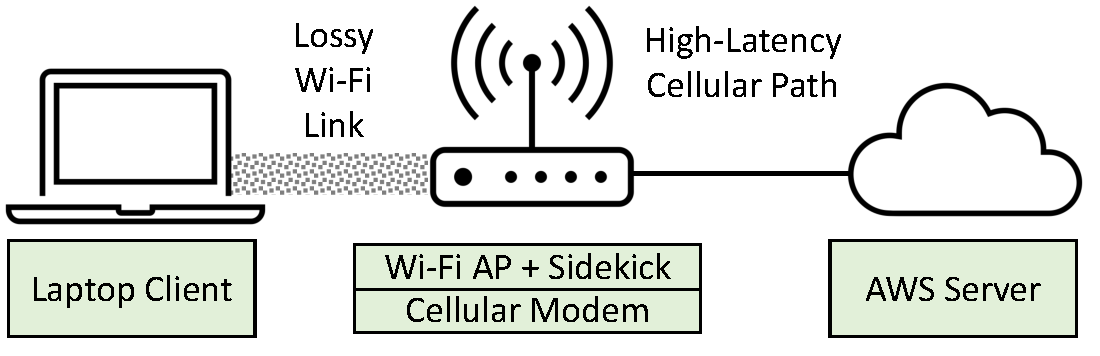
\includegraphics[width=\linewidth]{sidekick-paper/figures/setup_real.pdf}
\caption{Real-world experimental setup.
\vspace{-0.4cm}
}
\label{fig:setup:real}
\end{figure}


We modeled the scenarios from \Cref{sec:sidekick:motivating}. We use the same
m4.xlarge AWS instance as before for the emulated experiments.

\subsubsection{Emulation experiments.}

We emulated a two-hop network topology (\Cref{fig:sc-protocols}) in mininet,
configuring the link properties using \texttt{tc}.
In emulation, we represented
each link by a constant delay (with variability induced by the queue), a random
loss percentage, and a maximum bandwidth.
\Cref{tab:experimental-scenarios} describes the parameters
for each link to model---e.g., lossy Wi-Fi or a high-latency cellular
path---as well as the metrics for success in that scenario.
Link 1 connects the data sender (client) to the proxy,
while Link 2 connects the proxy to the data receiver (server).
On the proxy, we either run a Sidekick,
a connection-splitting TCP PEP~\cite{caini2006pepsal}, or nothing at all.

\subsubsection{Real-world experiments.}

To test its robustness, we also evaluated the Sidekick protocol over a real-world
environment that resembled the scenario on the train (\Cref{fig:setup:real}).
In this setup, a Lenovo ThinkPad laptop, running Ubuntu 22.04.3 with a 4-Core
Intel i7 CPU @ 2.60 GHz and 16 GB memory, acted as a client to an AWS instance in
the nearest geographical region. The ThinkPad used as an access point (AP)
a Lenovo Yoga laptop, running Ubuntu 20.04.6 with a 4-Core Intel i5 CPU @
1.60 GHz and 4 GB memory, with a 2.4 GHz Wi-Fi hotspot.
The AP was connected to the Internet via a JEXtream cellular modem
with a 5G data plan. The AP ran Sidekick software.

We measured the link properties of each path segment to compare to
our emulation parameters. We measured delay and loss using 1000~\texttt{ping}s
over a 100 second period, and bandwidth using an \texttt{iperf3} test.
On the near segment between the ThinkPad client and the AP,
the min/avg/max/stdev RTT was 1.249/37.194/272.168/54.660 ms
at 49.8 Mbit/s bandwidth. We observed that loss increased
the further away the AP. In our experiments, the client was located roughly
200 feet away in a different room, with 3.6\% loss.
The far segment between the AP and the AWS server was
48.546/64.381/92.374/6.806 ms with 0.0\% loss at 30.9 Mbit/s.
In both environments, the cellular link was the bottleneck link in terms of
bandwidth, and the corresponding path segments in emulation had similar
minimum RTTs and average loss percentages.

\section{Real-world results}
\label{sec:sidekick:real-world}

\begin{figure}[t]
\centering
\begin{subfigure}{0.48\linewidth}
	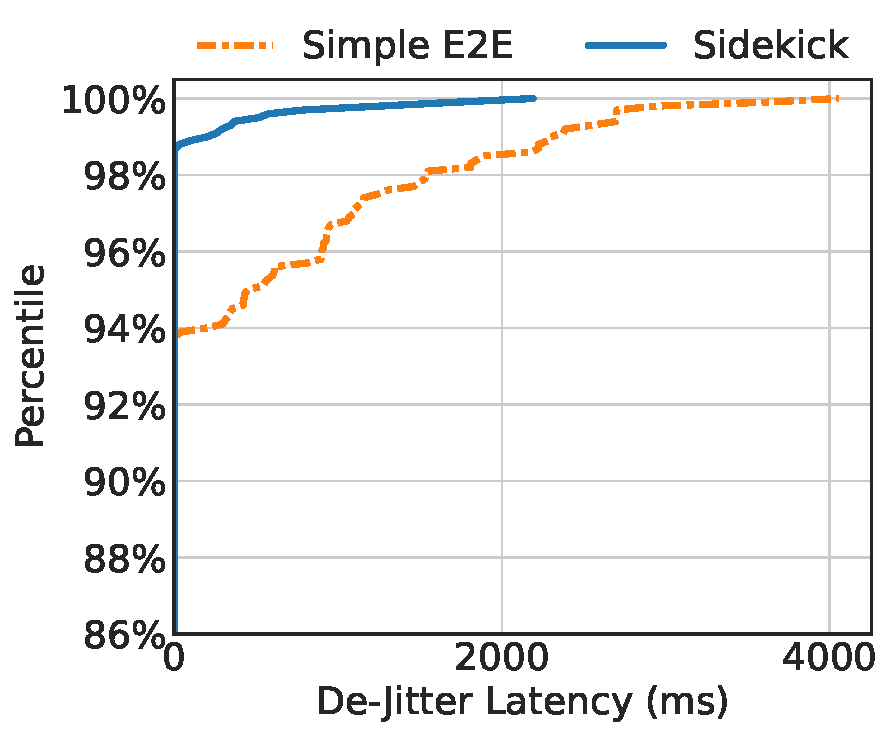
\includegraphics[width=\linewidth]{sidekick-paper/figures/fig8_real_world_webrtc.pdf}
	\caption{\footnotesize Low-latency media. CDF of per-packet de-jitter
	latencies over 10 one-minute trials per protocol.}
	\label{fig:real-world:scenario1}
\end{subfigure}
\begin{subfigure}{0.48\linewidth}
	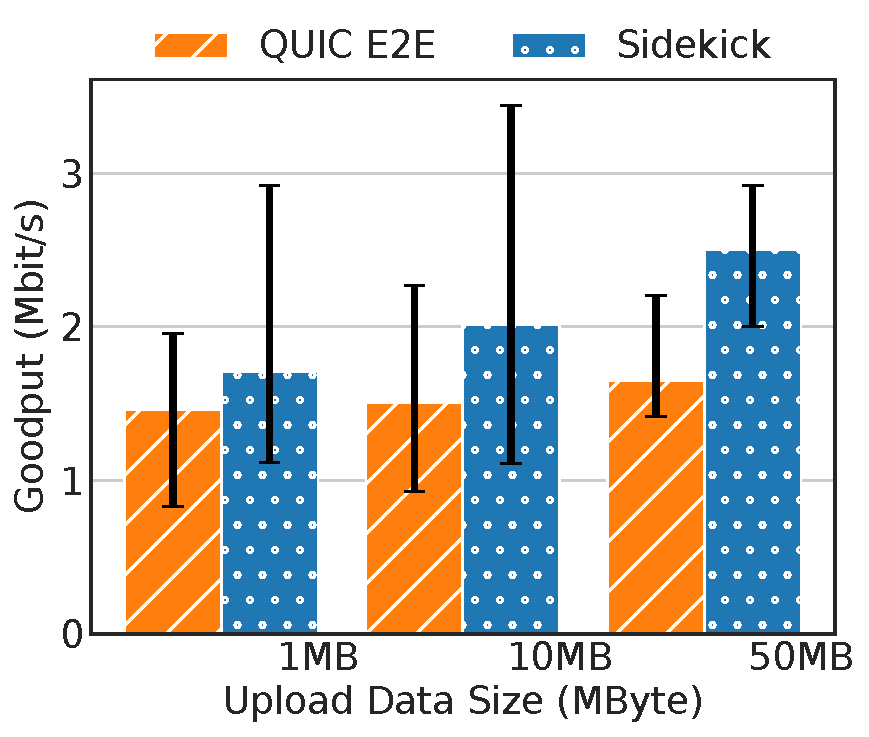
\includegraphics[width=\linewidth]{sidekick-paper/figures/fig8_real_world_retx.pdf}
	\caption{\footnotesize Path-aware congestion control.
	Median of 20 trials. Error bars are 1st and 3rd quartiles.}
	\label{fig:real-world:scenario2}
\end{subfigure}
\caption{Real-world results. Experiments were run in a moderately well-attended
office environment over a Friday afternoon. Trials alternate between the
baseline and the sidekick to account for variability in time of day.
}
\label{fig:real-world}
\end{figure}


We discuss the results of our experiments replicating two of our scenarios in
the real world, using as context
these main differences between emulation and the real-world:

\begin{itemize}[noitemsep,topsep=0pt]
  \item The RTT is more variable as it depends on interactions in the
  wireless medium and the shared cellular path.
  \item Wireless loss can be more variable as nearby 2.4 GHz devices and
  physical barriers may interfere with the link. Wireless loss also tends
  to be more clustered in practice.
  \item The available bandwidth on the shared cellular path is more variable,
  and depends on the time of day.
\end{itemize}

\Cref{fig:real-world} shows the results of running the low-latency media and
connection-splitting PEP emulation experiments in the real-world. The baseline
protocol with a Sidekick is able to
reduce the 99th percentile de-jitter latency of an audio stream
from 2.3~seconds to 204~ms---about a 91\% reduction---and
improve the goodput of a 50 MB HTTP/3 upload by about 50\%.
Although the improvements are more conservative compared to emulation in
\Cref{fig:media} and \Cref{fig:baseline-line}, each case still benefits the
base protocol under all circumstances, compared to end-to-end mechanisms alone.

Part of the difference can be attributed to the network setting. When there is
no loss on the near path segment, as can occasionally happen in a real Wi-Fi link,
we do not expect to
see a difference with a Sidekick. When there is more loss on the far path segment, which
is variable and depends on the time, we
expect the benefit of the Sidekick to be less since this equally affects the
performance of the base protocol.

The other part of the difference could be made up by future work that better
adapts a Sidekick connection to real-world variability: The client could improve
path segment RTT estimation based on when the proxy receives packets, and use this
dynamic estimate in the calculation of $r$ used in $\beta$ and $C$.
The client could also use
this estimate to dynamically adjust the quACK interval.
Finally, we could analyze theoretically how PACUBIC responds
to traffic patterns in the real world.

\section{Emulation results}
\label{sec:sidekick:emulation}

\begin{figure*}
% python latencies.py --percentile 99 --box-and-whiskers --http base quack_2p_8 -t 20
% python latencies.py --percentile 99 --box-and-whiskers -t 20
\begin{subfigure}{0.34\textwidth}
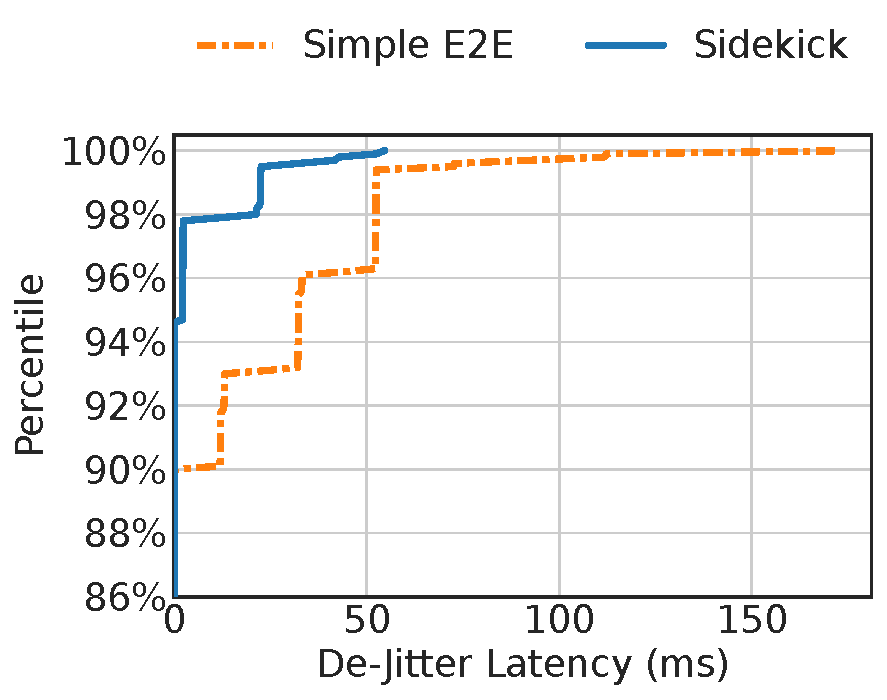
\includegraphics[width=\linewidth]{figures/fig4a_low_latency_media.pdf}
\caption{Scenario \#1: Low-latency media.
 Reduced tail latency of de-jitter delay
with earlier retransmission. 5 minute trials.}
\label{fig:media}
\end{subfigure}
\hfill
% python data_size_vs_tput.py --mean --median -t 10 --http quic quack_30ms_10 quack_60ms_20 quack_120ms_40
% python data_size_vs_tput.py --mean --median -t 10 --http quack_30ms_10 quic
\begin{subfigure}{0.31\textwidth}
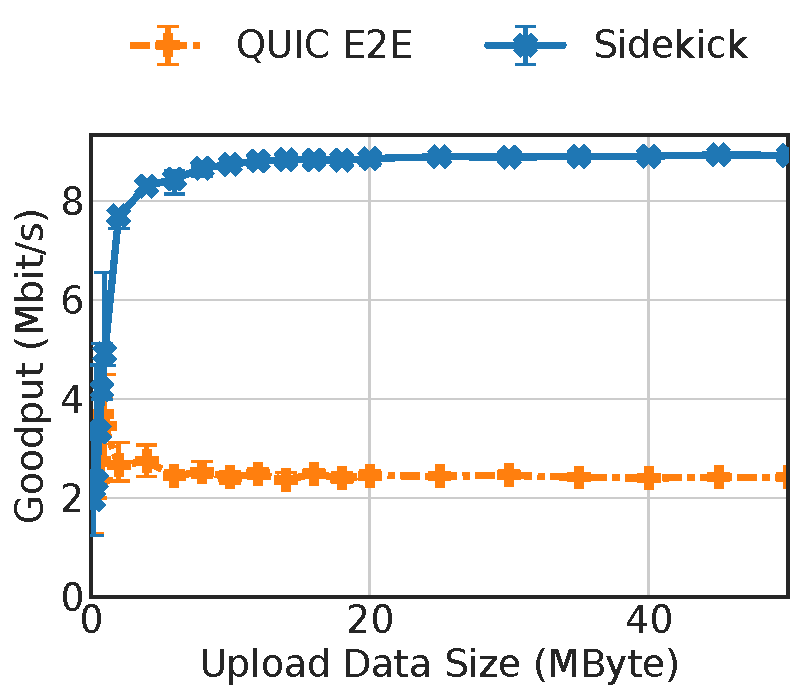
\includegraphics[width=0.97\linewidth]{figures/fig4b_pep_emulation.pdf}
\caption{Scenario \#2: Connection-splitting PEP emulation. Improved goodput.
20 trials median. Error bars are 1st and 3rd quartiles.
}
\label{fig:baseline-line}
\end{subfigure}
\hfill
\begin{subfigure}{0.32\textwidth}
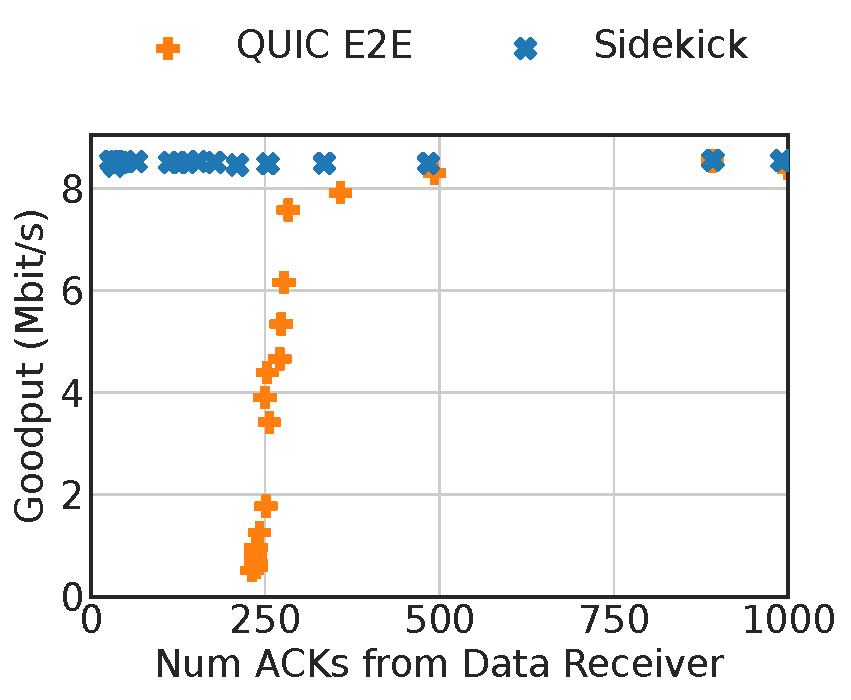
\includegraphics[width=0.99\linewidth]{figures/fig4c_ack_reduction.pdf}
\caption{Scenario \#3: ACK reduction.
High goodput independent of end-to-end ACK frequency.
10 MB upload.}
\label{fig:ack-reduction}
\end{subfigure}
\caption{
Comparing the end-to-end baseline protocol to the same protocol with a \sys
connection, using the success metrics for the three scenarios described in
\Cref{tab:experimental-scenarios}. The \textsf{\Sys($N$x)} data points show
the performance at $N$x the quACK interval (sent less frequently) and
threshold of the default configurations specified in
\Cref{tab:experimental-scenarios}.
\vspace{-0.3cm}
}
% \dm{Maybe a notation like $x/4$ would be more suggestive than $4x$?}
\label{fig:main-results}
\end{figure*}


We evaluated our implementation of the Sidekick protocol in a more controlled
emulation environment to answer the following questions:
\begin{enumerate}[noitemsep,topsep=0pt]
	\item Can Sidekicks improve the performance of secure transport protocols
	in a variety of scenarios while preserving the end-to-end behavior of the
	base protocols?
	\item Can a path-aware congestion control algorithm match the fairness of
	split TCP PEPs using CUBIC?
	\item How do the CPU overheads of encoding quACKs impact the maximum
	capacity of a proxy with a Sidekick?
	\item What link overheads does the power sum quACK add and how does it
	compare to the strawmen?
\end{enumerate}

\subsection{Performance of secure transport protocols with Sidekick}
\label{sec:sidekick:emulation:performance}

We first evaluate Sidekick's main performance goal: In each of the motivating
scenarios, we show that the Sidekick protocol can improve performance compared
to the base protocol alone, which would not be able to benefit from existing
PEPs. Each scenario has a different metric for success---tail latency,
throughput, or number of packets sent by the data receiver (corresponding to
energy usage or chance of Wi-Fi collisions)---demonstrating the versatility of
the Sidekick protocol.

\subsubsection{Low-latency media application.}
The Sidekick can reduce tail latencies in a low-latency media stream, representing
fewer drops and better quality of experience.
The early retransmissions induced by the Sidekick reduced the 99th percentile
latency of the de-jitter buffer delay from 48.6 ms to 2.2 ms---a 95\%
reduction (\Cref{fig:media}).
As long as the quACK interval is less than the end-to-end RTT, the connection
benefits from the Sidekick.

The Sidekick is beneficial in this scenario because it enables the client to sooner
detect and retransmit lost packets, and the server to sooner play packets from
its de-jitter buffer.
The end-to-end mechanism takes one additional received packet to notify of the
loss and
one end-to-end RTT to retransmit and play the packet (20+52=72ms), resulting in
three delayed packets (the three ``steps" in \Cref{fig:media}) in most cases.
The Sidekick takes up to two additional packets and one near path segment RTT
(20+2=22ms or 20$\times$2+2=42ms), delaying either one or two packets in comparison.
Dropped ACKs and quACKs account for the $<2\%$ of packets with even greater
de-jitter latencies.

\subsubsection{Connection-splitting PEP emulation.}
The Sidekick improves upload speeds when there is a lossy, low-latency link
by using quACKs to inform the sender's congestion control.
In a scenario with $1\%$ random loss on the link between the proxy and the
data sender, the HTTP/3 (QUIC) client achieves $3.6\times$ the goodput for a 10 MB
upload with a Sidekick compared to end-to-end QUIC (\Cref{fig:baseline-line}).

When there is no random loss, the Sidekick does not impact the performance
of QUIC\@.
There are no logical changes to the base protocol in this case because all loss
is on the
bottleneck link on the far path segment, and the CPU overheads of processing quACKs
are negligible.

Knowing \emph{where} congestion occurs is an opportunity for creating smarter
congestion control. In PACUBIC, identifying where the loss occured let the data
sender reduce the congestion window proportionally to how many packets were
in-flight on each path segment. In \Cref{sec:sidekick:emulation:pacubic}, we
will show that our path-aware congestion control algorithm still matches the
fairness of connection-splitting TCP PEPs.

\subsubsection{ACK reduction scenario.}

Using quACKs in lieu of end-to-end ACKs allows the data receiver to
significantly reduce its ACK frequency while maintaining high goodput.
In our experiment, QUIC with a Sidekick sent $96\%$ fewer packets (mainly ACKs)
than end-to-end QUIC before the goodput dropped below 8.5 Mbit/s
(\Cref{fig:ack-reduction}).
The quACK enables the data sender to promptly move the flow-control window forward,
as long as the last hop is reliable.

The goodput significantly degrades when reducing the end-to-end ACK frequency
without a Sidekick. When end-to-end QUIC reduces the ACK frequency to every
80 ms, the data receiver sends $247 / 138 = 1.8\times$ the packets at
$4.5 / 8.4 = 0.5\times$ the goodput, worse than QUIC with the Sidekick
in both dimensions (\Cref{fig:ack-reduction}). With a Sidekick,
the data sender also does not need to change packet pacing to avoid bursts in
response to infrequent ACKs, which is why end-to-end QUIC cannot send fewer
than $\approx 240$ packets.

\subsubsection{Discussion: Configuring the Sidekick connection.}
\Cref{tab:experimental-scenarios} shows the quACK interval and threshold we
elected for each scenario based on the considerations in
\Cref{sec:sidekick:init}. In each experiment in \Cref{fig:main-results},
we also show how with less frequent quACKs ($2\times$ and $4\times$ the
interval) and proportionally-adjusted thresholds, the protocol performs worse,
or more variably. Less frequent quACKs means the client reacts later to
feedback about the near path segment, and more often has to rely on the
end-to-end mechanism. The performance particularly degrades when the quACK
interval exceeds the end-to-end RTT. However, even in this case, the base
protocol with any Sidekick at all performs better than the base protocol alone\@.

\subsection{Link overheads from sending quACKs}
\label{sec:sidekick:emulation:link-overheads}

\begin{figure}[h]
\begin{subfigure}{\columnwidth}
  % 5+
  %
  \setlength{\tabcolsep}{2pt}
  \footnotesize
  \centering
  \begin{tabular}{lccccccc}
    \toprule
    & \multicolumn{2}{c}{Data Sender$\rightarrow$} & \multicolumn{2}{c}{$\leftarrow$Proxy} & \multicolumn{2}{c}{$\leftarrow$Data Receiver} & \\
    & \bf Pkts & \bf Bytes & \bf Pkts & \bf Bytes & \bf Pkts & \bf Bytes & \bf Goodput \\
    \midrule
    QUIC E2E & $1.00\times$ & $1.00\times$ & $1.00\times$ & $1.00\times$ & $1.00\times$ & $1.00\times$ & $1.00\times$ \\
    Strawman 1a & $0.96\times$ & $1.01\times$ & \cellcolor{LighterRed}{$2.02\times$} & \cellcolor{LightestRed}{$1.56\times$} & $1.01\times$ & $1.03\times$ & \cellcolor{LighterGreen}{$3.33\times$} \\
    Strawman 1b & $0.94\times$ & $1.00\times$ & \cellcolor{LighterRed}{$2.00\times$} & \cellcolor{LightestRed}{$1.78\times$} & $1.00\times$ & $1.03\times$ & \cellcolor{LightGreen}{$3.53\times$} \\
    Strawman 1c & \cellcolor{LightestRed}{$1.83\times$} & $1.06\times$ & \cellcolor{LighterRed}{$2.01\times$} & \cellcolor{LightestRed}{$1.83\times$} & $1.00\times$ & $1.03\times$ & \cellcolor{LightGreen}{$3.46\times$} \\
    \bf \textcolor{black!50!blue}{Power Sum}   & \textcolor{black!50!blue}{\bf 0.94$\times$} & \textcolor{black!50!blue}{\bf 1.00$\times$} & \textcolor{black!50!blue}{\bf 1.03$\times$} & \textcolor{black!50!blue}{\bf 1.07$\times$} & \textcolor{black!50!blue}{\bf 1.00$\times$} & \textcolor{black!50!blue}{\bf 1.03$\times$} & \cellcolor{LightGreen}{\textcolor{black!50!blue}{\bf 3.55$\times$}} \\
    \bottomrule
  \end{tabular}
  % \includegraphics[width=\columnwidth]{figures/packet-overhead-retx.png}
  \caption{Scenario \#2: Connection-splitting PEP emulation.}
  \label{tab:packet-overhead:retx}
\end{subfigure}
\begin{subfigure}{\columnwidth}
  % \includegraphics[width=\columnwidth]{figures/packet-overhead-ackr.png}
  \setlength{\tabcolsep}{2pt}
  \footnotesize
  \centering
  \begin{tabular}{lccccccc}
    \toprule
    & \multicolumn{2}{c}{Data Sender$\rightarrow$} & \multicolumn{2}{c}{$\leftarrow$Proxy} & \multicolumn{2}{c}{$\leftarrow$Data Receiver} & \\
    & \bf Pkts & \bf Bytes & \bf Pkts & \bf Bytes & \bf Pkts & \bf Bytes & \bf Goodput \\
    \midrule
    QUIC E2E & $1.00\times$ & $1.00\times$ & $1.00\times$ & $1.00\times$ & $1.00\times$ & $1.00\times$ & $1.00\times$ \\
    Strawman 1a & $0.96\times$ & $1.00\times$ & \cellcolor{LightRed}{$9.94\times$} & \cellcolor{LighterRed}{$4.99\times$} & \cellcolor{LightGreen}{$0.04\times$} & \cellcolor{LightGreen}{$0.08\times$} & $1.02\times$ \\
    Strawman 1b & $0.96\times$ & $1.00\times$ & \cellcolor{LightRed}{$9.95\times$} & \cellcolor{LightRed}{$7.13\times$}      & \cellcolor{LightGreen}{$0.04\times$} & \cellcolor{LightGreen}{$0.08\times$} & $1.02\times$ \\
    Strawman 1c & \cellcolor{LightestRed}{$1.91\times$} & $1.05\times$ & \cellcolor{LightRed}{$9.73\times$} & \cellcolor{LightRed}{$7.41\times$}      & \cellcolor{LightGreen}{$0.04\times$} & \cellcolor{LightGreen}{$0.08\times$} & $0.97\times$ \\
    \bf \textcolor{black!50!blue}{Power Sum}    & \textcolor{black!50!blue}{\bf 0.96$\times$} & \textcolor{black!50!blue}{\bf 1.00$\times$} & \textcolor{black!50!blue}{\bf 1.09$\times$} & \cellcolor{LighterRed}{\textcolor{black!50!blue}{\bf 2.56$\times$}} & \cellcolor{LightGreen}{\textcolor{black!50!blue}{\bf 0.04$\times$}} & \cellcolor{LightGreen}{\textcolor{black!50!blue}{\bf 0.08$\times$}} & \textcolor{black!50!blue}{\bf 0.98$\times$} \\
    \bottomrule
  \end{tabular}
  \caption{Scenario \#3: ACK reduction.}
  \label{tab:packet-overhead:ackr}
\end{subfigure}
\caption{Link overheads for a 10 MB upload. The cells represent the multiplier
relative to the end-to-end QUIC baseline for each type of quACK\@.
Lower is better for number of packets and bytes sent on a link.
Higher goodput is better. Robin's power sum quACK achieves the success metric
for each scenario without incurring the link overheads of the strawmen.
We did not evaluate the contrived protocol in Scenario \#1.
}
\label{tab:packet-overhead}
\end{figure}


The other cost in terms of using Sidekick protocols is the additional data
sent by the proxy to the data sender.
Too many additional bytes use up bandwidth, and additional packets use
up CPU\@.
\Cref{tab:packet-overhead} shows the number of packets and bytes sent at each
node comparing the strawmen and power sum quACK to no Sidekick connection at all.

Using power sum quACKs increases the packets sent from the proxy to the data
sender
by 3-9\%. These packets either consist mostly
of end-to-end ACKs which are sent every packet in \texttt{quiche}, or end-to-end
ACKs that have been replaced by quACKs in the ACK reduction scenario.
We did not evaluate Scenario \#1 because it is based
on a contrived protocol that lacks many of these features, and the link
overheads would not really make sense.

This overhead is representative of the CPU overhead at the client, since
quACKs and ACKs take a similar number of cycles to process. In an experiment
with Scenario \#2 during a period of $\approx90$k incoming packets, ACKs took on
average 26065 cycles to process while the quACKs took 26369 cycles, 1\% more.
These cycles come from, i.e., the complex recovery and loss detection algorithms
implemented at the end host.

The strawmen have significantly higher link overheads compared to the power sum
quACK\@. The proxy sends up to 10$\times$ more packets using Strawman 1a, and
also slightly harms the goodput in the congestion control scenario.
The reduced goodput is due to the sender mis-identifying received packets as
dropped due to dropped quACKs.
The proxy achieves higher goodput with Strawman 1b but sends
more bytes. Strawman 1c increases the link overheads at both the proxy and the
data sender due to larger TCP headers and TCP ACKs.
We did not evaluate Strawman 2 due to its impractical decode time.

\subsection{CPU overheads of encoding at the proxy}
\label{sec:sidekick:emulation:cpu-overheads}

\begin{table}[ht]
  \centering
  \small
  \begin{tabular}{lrrrr}
    \toprule
    & \multicolumn{2}{r}{\bf 25-Byte Payload} & \multicolumn{2}{r}{\bf 1468-Byte Payload}\\
    & \bf Cycles & \bf $\%$ & \bf Cycles & \bf $\%$ \\
    \midrule
    Sniff Packet & 22417 & 97.6 & 22408 & 97.5 \\
    Table Lookup &   247 &  1.1 &   251 &  1.1 \\
    Parse ID     &    23 &  0.1 &    22 &  0.1 \\
    Encode ID    &    74 &  0.3 &    69 &  0.3 \\
    Other        &   213 &  0.9 &   225 &  1.0 \\
    \midrule
    \emph{Total} & \emph{22974} & \emph{100.0} & \emph{22975} & \emph{100.0} \\
    \bottomrule
  \end{tabular}
  \caption{Breakdown of the CPU cycles spent processing each packet at the
  proxy. Most cycles are spent on general per-packet overheads as opposed to
  quACK-specific processing.
  }
  \label{tab:cpu-overhead}
\end{table}


The main bottleneck of Sidekick on a proxy is the CPU\@.
\Cref{tab:cpu-overhead} shows a breakdown of the number of CPU cycles in each
step. The largest overhead was reading the packet contents from the network
interface ($97.5\%$ of the CPU cycles).

Encoding an identifier in a power sum quACK with $t=10$ used $74$ CPU
cycles ($0.9\%$). As a calculation of the theoretical maximum on a 2.30 GHz
% 2.30e9 / 74 = 31 million
CPU, the proxy would be able to process $31$ million packets/second on a single
core. The hash table lookup used $251$ cycles and parsing the pseudorandom
payload as an identifier used $22$ cycles.

In practice, we measured the maximum throughput of our Sidekick proxy to
be 464k packets/s with 25-byte payloads and 5.5 Gbit/s (458k packets/s) with
1468-byte packet payloads on a single core (assuming 1500-byte MTUs).
This experiment used multiple \texttt{iperf3} clients to simulate high
load until the proxy was unable to keep up with the load on a single core.
The packet payload size did not seem to affect results.

We find these achieved throughputs acceptable for edge routers such as Wi-Fi APs
and base stations. To deploy the Sidekick proxy on core routers, we would need
to reduce the overhead of reading packets from the NIC, such as by bypassing
the kernel/user-space protection boundary\footnote{ A kernel-bypass system like
Retina~\cite{wan2022retina} can achieve 25 Gbps on 2 cores while processing raw
packets with a 1000-cycle callback(Figure 5(a) in \cite{wan2022retina}). The
Sidekick equivalent would be a 500-cycle callback, and assuming all traffic has
requested Sidekick help. Throughput scales almost linearly with the number of
cores using symmetric RSS hashing. Thus we don't expect proxy overheads to be
an issue with modern 100 Gbps network speeds and an optimized implementation
even on commodity hardware. }~\cite{dpdk,mccanne1993bsd,wan2022retina} or using
native hardware~\cite{bosshart2014p4}. We could also scale on multiple cores
using symmetric RSS hashing~\cite{woo2012scalable}.

\subsection{TCP friendliness of path-aware CUBIC}
\label{sec:sidekick:emulation:pacubic}

\begin{figure}[t]
\centering

\includegraphics[width=\columnwidth]{figures/fig5_baseline_bar_legend.pdf}
\begin{subfigure}{0.49\linewidth}
	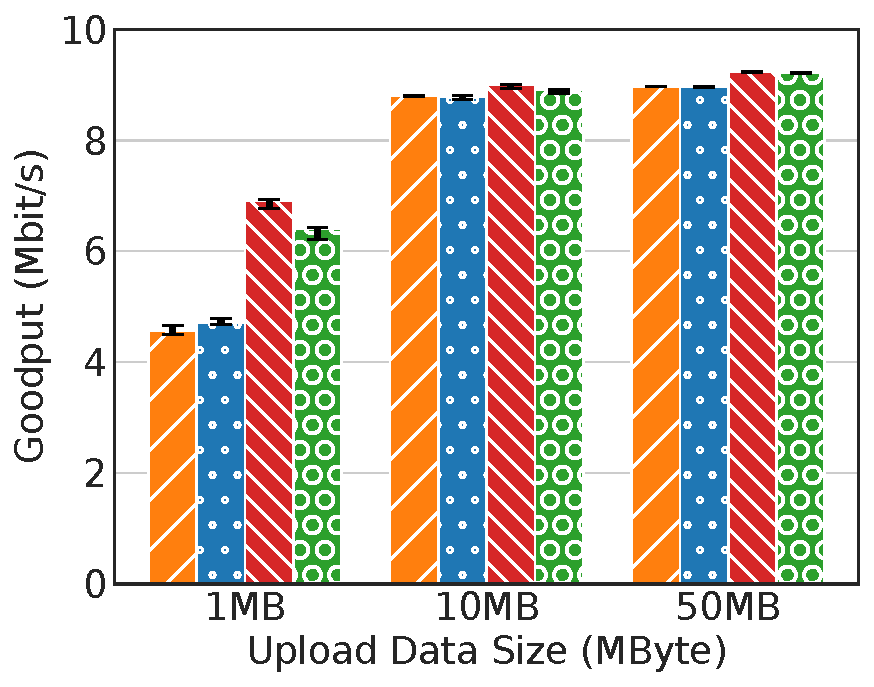
\includegraphics[width=\linewidth]{figures/fig5_baseline_loss0p.pdf}
	\caption{0\% loss.}
	\label{fig:baseline-bar:loss0p}
\end{subfigure}
\begin{subfigure}{0.49\linewidth}
	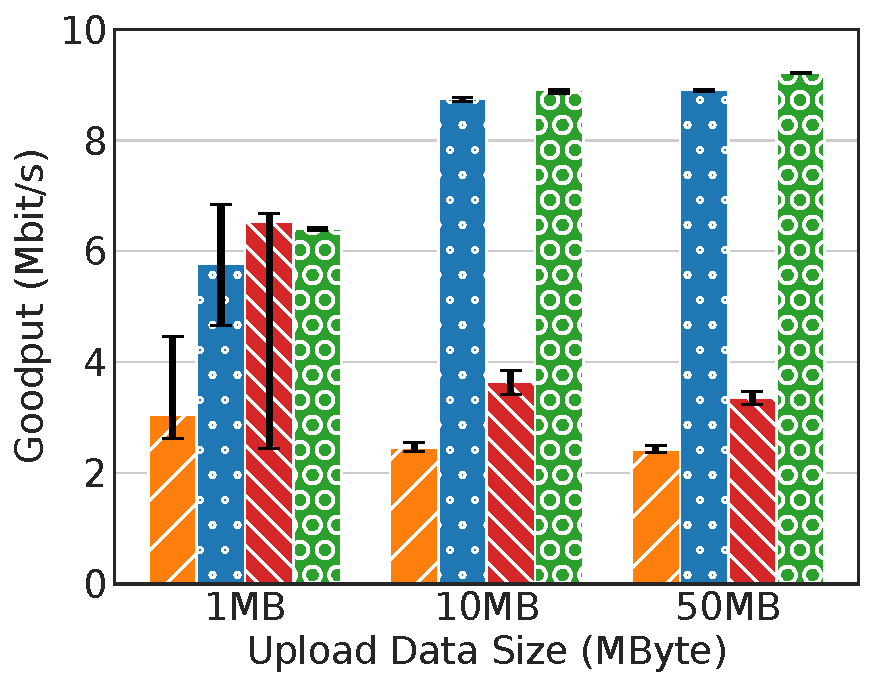
\includegraphics[width=\linewidth]{figures/fig5_baseline_loss1p.pdf}
	\caption{1\% loss.}
	\label{fig:baseline-bar:loss1p}
\end{subfigure}
\vspace{-0.2cm}
\caption{Median goodput for three upload data sizes with $0\%$ and $1\%$ loss on
Link 1. 20 trials. Error bars are 1st and 3rd quartiles.
With proxy assistance at $1\%$
loss, both QUIC and TCP match the performance of when there is no loss at all.
\vspace{-0.4cm}
}
\label{fig:baseline-bar}
\end{figure}

\begin{figure}[t]
\centering
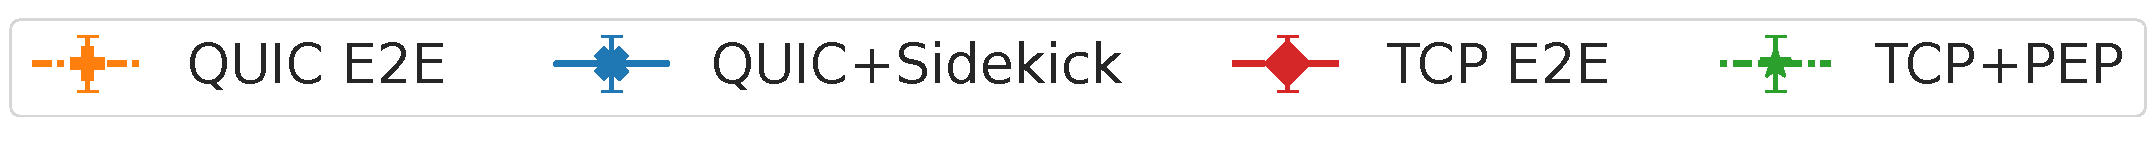
\includegraphics[width=\columnwidth]{figures/fig6_legend.pdf}
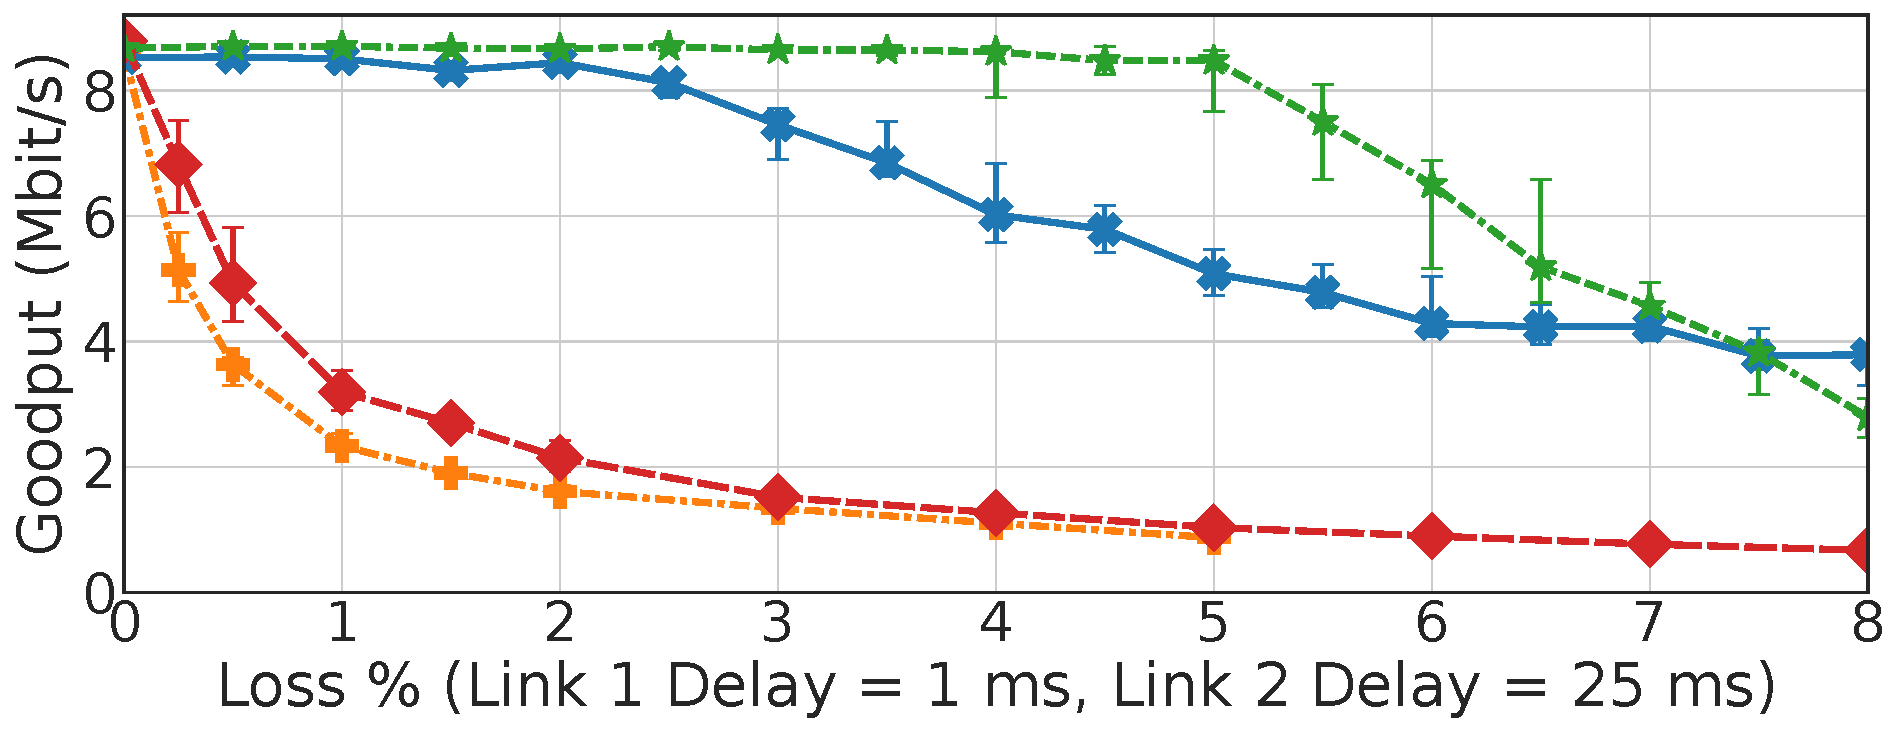
\includegraphics[width=\columnwidth]{figures/fig6_loss_bw100_10M_delay_25ms_1ms.pdf}
%\includegraphics[width=\columnwidth]{figures/loss_bw100_10M_delay_15ms_11ms.pdf}
\vspace{-0.4cm}
\caption{Connection-splitting PEP emulation as a function of near-segment
	loss rate. In this emulation experiment, QUIC+\Sys (running PACUBIC)
  performs similarly to TCP+PEP (each connection running CUBIC)
  and improves goodput compared with end-to-end protocols. The graph shows
  median goodput of a 10~MByte upload. QuACK interval is 30~ms, threshold
is 10. Error bars show IQR of 10 trials.
\vspace{-1cm}
}
\label{fig:loss-vs-tput}
\end{figure}

%\begin{figure}[t]
%\centering
%	\includegraphics[width=0.6\linewidth]{figures/multiflow_loss0p_legend.pdf}\\
%	\includegraphics[width=0.32\linewidth]{figures/quic_quack_60M_loss0p_delay0s_bw100.pdf}
%	\includegraphics[width=0.32\linewidth]{figures/quic_quack_60M_loss0p_delay5s_bw100.pdf}
%	\includegraphics[width=0.32\linewidth]{figures/quack_quic_60M_loss0p_delay5s_bw100.pdf}
%        \caption{Fairness evaluation of two concurrent QUIC flows in
%          Scenario \#1 (but without loss on the near path segment), one \sys-assisted and one end-to-end, in a purely
%          congestion-limited situation. The use of
%          \sys assistance doesn't affect 
%
%          Throughput of two concurrent flows in Scenario 1 (with $0\%$ and $1\%$
%loss on Link 1. Both flows converge to a steady-state throughput, whether the
%flows start at the same time (left) or at a 5 second delay (middle, right).}
%\label{fig:multiflow}
%\end{figure}

% \begin{figure*}
% \centering
% \includegraphics[width=\columnwidth]{figures/legend.pdf}\\
% \subfigure[QUIC, QUIC no delay]{
% 	\includegraphics[width=0.185\textwidth]{figures/quic_quic_60M_loss0p_delay0s.pdf}
% 	\label{fig:multiflow:a}}
% \subfigure[QUIC, QUIC 5s delay]{
% 	\includegraphics[width=0.185\textwidth]{figures/quic_quic_60M_loss0p_delay5s.pdf}
% 	\label{fig:multiflow:b}}
% \subfigure[QUIC, \sys no delay]{
% 	\includegraphics[width=0.185\textwidth]{figures/quic_quack_60M_loss0p_delay0s.pdf}
% 	\label{fig:multiflow:c}}
% % \subfigure[quack, quic no delay]{
% % 	\includegraphics[width=0.185\textwidth]{figures/quack_quic_60M_loss0p_delay0s.pdf}}
% \subfigure[QUIC, \sys 5s delay]{
% 	\includegraphics[width=0.185\textwidth]{figures/quic_quack_60M_loss0p_delay5s.pdf}
% 	\label{fig:multiflow:d}}
% \subfigure[\sys, QUIC 5s delay]{
% 	\includegraphics[width=0.185\textwidth]{figures/quack_quic_60M_loss0p_delay5s.pdf}
% 	\label{fig:multiflow:e}}
% % \label{fig:multiflow:quic-quack}
% % \end{figure*}

% % \begin{figure*}
% % \centering
% \subfigure[PEP, PEP no delay]{
% 	\includegraphics[width=0.185\textwidth]{figures/pep_pep_60M_loss1p_delay0s.pdf}
% 	\label{fig:multiflow:f}}
% \subfigure[PEP, PEP 5s delay]{
% 	\includegraphics[width=0.185\textwidth]{figures/pep_pep_60M_loss1p_delay5s.pdf}
% 	\label{fig:multiflow:g}}
% \subfigure[PEP, \sys no delay]{
% 	\includegraphics[width=0.185\textwidth]{figures/pep_quack_60M_loss1p_delay0s.pdf}
% 	\label{fig:multiflow:h}}
% % \subfigure[quack, pep no delay]{
% % 	\includegraphics[width=0.185\textwidth]{figures/quack_pep_60M_loss1p_delay0s.pdf}}
% \subfigure[PEP, \sys 5s delay]{
% 	\includegraphics[width=0.185\textwidth]{figures/pep_quack_60M_loss1p_delay5s.pdf}
% 	\label{fig:multiflow:i}}
% \subfigure[\sys, PEP 5s delay]{
% 	\includegraphics[width=0.185\textwidth]{figures/quack_pep_60M_loss1p_delay5s.pdf}
% 	\label{fig:multiflow:j}}
% \caption{Multiflow experiment with various combinations of QUIC end-to-end and QUIC+\sys at 0\% loss (a-e),
% and various combinations of TCP+PEP and QUIC+\sys at 1\% loss (f-j), demonstrating
% flow fairness. The delay indicates how long we started the second flow after the first flow.}
% \label{fig:multiflow}
% \end{figure*}


It is easy to improve performance without regard to competing flows;
however, we demonstrate that PACUBIC can
match the fairness of split CUBIC in a TCP PEP connection\@.
We evaluate fairness using Scenario \#2 with varying amounts of loss on the
near path segment.

\subsubsection{QUIC vs.\ TCP\@.}
We first compare QUIC to TCP without either PEP\@.
As both connections use CUBIC, they exhibit similar
congestion control behavior and achieve nearly maximum throughput in the
emulated network with no random loss (\Cref{fig:baseline-bar:loss0p}).
We attribute the differences to the slightly different retranmission and
loss recovery behaviors of QUIC and TCP\@. The PEPs do not affect the
performance.

With even a little loss on the near path segment, both QUIC and TCP dramatically
worsen, respectively achieving $28\%$ and $42\%$ of the goodput at $0\%$ loss,
for a 10 MB upload (\Cref{fig:baseline-bar:loss1p}).
% 0.305 / 1.098 = 27.8%
% 0.467 / 1.121 = 41.7%
In both protocols, CUBIC treats every transmission error as a congestion event,
even though no amount of reducing the congestion window affects the error rate.
QUIC and TCP perform similarly to each other with proxy assistance and 1\%
loss on the near path segment.

\subsubsection{Sidekick vs.\ TCP PEP\@.}
\Cref{fig:loss-vs-tput} shows that QUIC with a Sidekick roughly matches---as
 intended---the behavior of TCP with a PEP-assisted split connection. At higher
loss rates, the near path segment becomes the bottleneck link even with earlier
feedback about loss, causing the performance of TCP with proxy assistance to
drop. QUIC with a Sidekick follows a similar pattern because of its path-aware
congestion-control scheme (\Cref{sec:sidekick:sender}). The
results indicate that the Sidekick protocol's gains do not come at the expense
of congestion-control fairness relative to the split TCP connection.
